\documentclass[10pt,sigconf,letterpaper]{acmart}

\renewcommand\footnotetextcopyrightpermission[1]{} % 
%removes footnote with conference info
\setcopyright{none}
\settopmatter{printacmref=false, printccs=false, 
printfolios=false}
\pagestyle{plain}


%\documentclass[10pt,sigconf,letterpaper]{acmart}
\usepackage{color}
%\usepackage[nolist]{acronym}
%\usepackage{amsmath,amssymb}
\usepackage{pifont}
%\usepackage{enumitem}
%\usepackage{booktabs}
%\usepackage{graphicx} % embedded graphics
%\usepackage{url}
\usepackage{xcolor}
%\usepackage{times}  % Times fonts look better
%\usepackage{array}  % Extended styles for tables
%\usepackage{textcomp}

% \iffalse
\iftrue
\newcommand{\randall}{\ding{110}\ding{43}\textcolor{magenta}}
\newcommand{\pes}{\ding{110}\ding{43}\textcolor{blue}}
\newcommand{\geoff}[1]{\ding{110}\ding{43}\textcolor{violet}{#1}}
\else
\newcommand{\randall}{}
\newcommand{\pes}{}
\newcommand{\geoff}[1]{}
\fi

%\DeclareFontFamily{\encodingdefault}{\ttdefault}{\hyphenchar\font=`\-}

% \setcopyright{acmcopyright}
% \copyrightyear{2018}
% \acmYear{2018}
% \acmDOI{10.1145/1122445.1122456}

%\copyrightyear{2022}
%\acmYear{2022}
%\acmConference[IMC '22]{Internet Measurement 
%Conference}{October 25--27, 2022}{Nice, France}
\acmConference{}{}{}
%\acmBooktitle{Internet Measurement Conference (IMC '22), 
%October 25--27, 2022, Nice, France}
%\acmPrice{TBA}

\begin{document}

%\author{Submission \#19}
%\author{Audrey Randall}
%\email{aurandal@eng.ucsd.edu}
%\affiliation{UC San Diego}
%\author{Peter Snyder}
%\email{pes@brave.com}
%\affiliation{Brave Software}
%\author{Alisha Ukani}
%\email{aukani@ucsd.edu}
%\affiliation{UC San Diego}
%\author{Alex Snoeren}
%\email{snoeren@cs.ucsd.edu}
%\affiliation{UC San Diego}
%\author{Geoffrey M.\ Voelker}
%\email{voelker@cs.ucsd.edu}
%\affiliation{UC San Diego}
%\author{Stefan Savage}
%\email{savage@cs.ucsd.edu}
%\affiliation{UC San Diego}
%\author{Aaron Schulman}
%\email{schulman@cs.ucsd.edu}
%\affiliation{UC San Diego}

\title{The Challenges Associated With Decentralized Naming for Legal Takedowns}
%\renewcommand{\shortauthors}{A. Randall \textit{et al.}}

%\runningtitle{Article title}

%\subtitle{...}

%\abstract{stuff?}


\maketitle
\pagestyle{plain}

\section{Introduction}

\begin{itemize}
	\item Malware uses DNS to reach CNC servers. 
	\begin{itemize}
		\item Malware needs a naming layer because of the 
		sunk infrastructure cost: 
		any malware already deployed that uses an IP that gets blocked/taken 
		over is now useless. Malware authors want a record they can change.
		\item Naming layer needs to be hard to block at both 
		the request level and the system level, so that 
		already-distributed malware doesn't lose access and 
		become useless. 
	\end{itemize}
	\item DNS is decentralized in that there are many resolvers, but 
	centralized in that there are centralized authorities. Defenders can serve 
	legal takedown notices to those centralized authorities to block malware's 
	access to its CNC servers.
	\item Pivot: Malware is starting to use a truly decentralized naming 
	system, ``blockchain DNS.'' This creates several challenges for defenders:
	\begin{itemize}
		\item No central authority is capable of enacting domain-level takedown 
		orders
		\item For large chains, there is enough legitimate content that 
		blocking access to the whole chain is infeasible
		\item Transactions on large chains cost a lot of money. This limits 
		defenders' abilities to stage interventions like pre-registering all 
		domains listed in a malware's DGA.
	\end{itemize}
	\item We study the ecosystem and point out several places where 
	interventions are still possible, and discuss the challenges to defenders 
	and occasional advantages they gain when malware uses decentralized naming 
	such as blockchain DNS.
\end{itemize}

\section{Background}

\randall{this is so terrible but you can't edit a blank page}

To control a large number of infected hosts, malware often requires a command and control (C2) 
center 
to send commands or provide a location to upload data. 
The C2 center, as a single point of failure, presents an obvious weak link for defenders to target, 
so 
malware authors want to preserve the ability to change its location if it gets taken down. This 
means 
that infected hosts must remain able to contact the C2 center even if 
its address is changed. If defenders take down a C2 center, and the infected hosts that relied on 
it 
cannot find a new C2 center, those infected clients become useless. Malware authors must therefore 
avoid a ``sunk cost'' problem, where they deploy code that knows to contact a C2 center at a 
certain 
location, but then lose the ability to use or update those hosts when the C2 center is taken down.

To ensure that hosts remain able to contact C2 centers, modern malware generally does not hard-code 
the address of the C2 center directly into the deployed code. Instead, malware authors need to 
provide 
a layer of indirection --- a naming layer --- so that deployed malware can have a 
fixed, hard-coded destination to reach out to to get further instructions. 
This naming layer should be resilient to takedown efforts.

\subsection{What features of naming systems are desirable for storing C2 domain names?}

From a malware author's perspective, an ideal naming system for recording C2 
addresses is uncensorable at both the request level and the system level. To be 
uncensorable at the request level, there should be no central authority that 
has the ability to enforce a legal takedown notice for an individual record. To 
be uncensorable at the system level, the system should be valuable enough to 
licit actors that authorities cannot block access to it entirely without 
causing significant collateral damage to benign users.

To some extent, a trade-off exists between these features. On 
one side of the 
spectrum, protocols like Tor provide high resistance to request-level 
censorship, but they stand out, allowing systems like IDSes to detect the 
malware's presence.
%but do not have enough licit traffic to prevent authorities from 
%blocking access to the system entirely. \randall{Cite that paper that   
%said when you take away the malware, what's left is 80\% CSAM, and find other 
%citations that say defenders block Tor.}
On the other side of 
the scale, malware has repurposed ubiquitous, benign systems 
such as social media to store C2 addresses. Defenders do not 
want to impose blanket bans on applications accessing social 
media URLs, but social media companies such as Facebook and 
Twitter have the capability, motivation, and legal obligation to enforce 
legal takedown requests on individual posts. 

\subsection{DNS-based domain names}

Traditional DNS has high system-level resistance to censorship but low request-level resistance. 
Since 
nearly every device and application on the Internet requires DNS, enterprises and firewalls almost 
never block it entirely. However, while DNS is a decentralized system in terms of how its 
components 
are replicated across the globe, it is not decentralized in terms of authority. The registrar 
that sold a domain can be compelled to ``delete'' that domain or prevent it from being updated or 
transferred. 

The usual process for enacting a legal takedown in the United States works as 
follows~\cite{knight_domain_2015}. Upon 
identifying a domain that is being used as a C2 center, a law enforcement entity may choose to make 
an Acceptable Use Policy (AUP) complaint or may immediately seek a court order compelling the 
registrar to take down the domain. Some registrars cooperate with AUC complaints without legal 
intervention, but others do not. If the registrar does not respond to the AUC complaint and take 
down the domain, law enforcement may move on to using a court order. The court order commonly 
prevents the domain from being updated or transferred rather than deleting it entirely, because if 
the domain is deleted, it can be re-registered. The court order also specifies whether the domain 
should continue to resolve, resolve to a new IP address specified by the order, or stop resolving 
altogether. 

Court orders may be obtained by civil parties as well. The most common method is for a company to 
apply for a temporary restraining order (TRO), which orders the perpetrators of the offending 
activity to cease and desist and requires any intermediaries that provide services to the 
perpetrators to cease providing those services~\cite{kesari_deterring_2017}. The latter requirement 
is what allows companies to require registrars to ``sinkhole'' C2 domains. 

\subsection{Blockchain-based domain names}

Blockchain-based naming systems present a potential threat 
because they can provide 
both qualities: they are difficult to censor at the request 
level as well as the system level. Blockchains are designed 
to prevent anyone from changing a record once it has been 
created, except for the record's owner. No central authority 
controls blockchain domains in the same way that registrars 
control traditional DNS names. Thus, even the companies 
selling blockchain domains do not have the capability to 
comply with a legal takedown request. Furthermore, even if a 
domain owner changes a domain record, the previous record 
will still be available on the chain: it cannot be deleted. 
Furthermore, some blockchains, such as Bitcoin and Ethereum, have recently 
skyrocketed in popularity as investors became interested in cryptocurrency as 
an asset class. Because these blockchains are no longer niche systems of 
interest only to a small group of technologically-savvy users, blocking access 
to them entirely will be impossible without angering a large number of 
legitimate users. As far as we are aware, cryptocurrencies and the blockchains 
they rely on are the first examples of strongly censorship-resistant systems 
that have gained a substantial community of legitimate users around the world.

Therefore, blockchain is likely to get used more in the future as a naming 
layer for the addresses of CNC servers. In fact, we already see some malware 
using it. However, blockchain is not as invincible as it claims. (summary of 
examples?)

In the remainder of this work, we detail the specific 
challenges posed by the blockchain DNS ecosystem to malware 
defenders, as well as the pieces of the ecosystem where 
effective interventions might be staged.

%Blockchains provide two censorship-resistant properties that 
%are desirable to malware authors. First, once a record 
%is created on the chain and sufficient blocks have been added 
%on top of it, it can only be updated by its owner. 
%Second, a client can access the entire blockchain as long as 
%it can reach a single participating node. However, blockchain 
%ecosystems still provide opportunities for defenders to stage 
%interventions against malware: most notably, when malware 
%connects to the chain for the first time. 


%the censorship-resistant properties of blockchains are only 
%guaranteed for transactions on the chain itself. 

%Blockchains typically present two challenges---usability and 
%performance---that incentivize users to introduce off-chain, 
%centralized authorities into the ecosystem. These 
%centralized 
%authorities can be legally compelled to enact takedown 
%requests. For example, most users connect to blockchains via 
%centralized proxies rather than by running their own nodes, 
%because running a node typically involves significant energy 
%and hardware resources. Additionally, many current users of 
%blockchain DNS domains store their records on chain in the 
%form of traditional DNS domains, rather than IP addresses. 
%These traditional domains are subject to the authority of 
%the 
%registrars that issued them. Some chains also present a 
%third 
%challenge: the high monetary cost of transactions, which 
%makes creating and updating records difficult for malware 
%authors and defenders alike. 


\section{Accessing records}

\begin{figure*}[t]
	\centering
	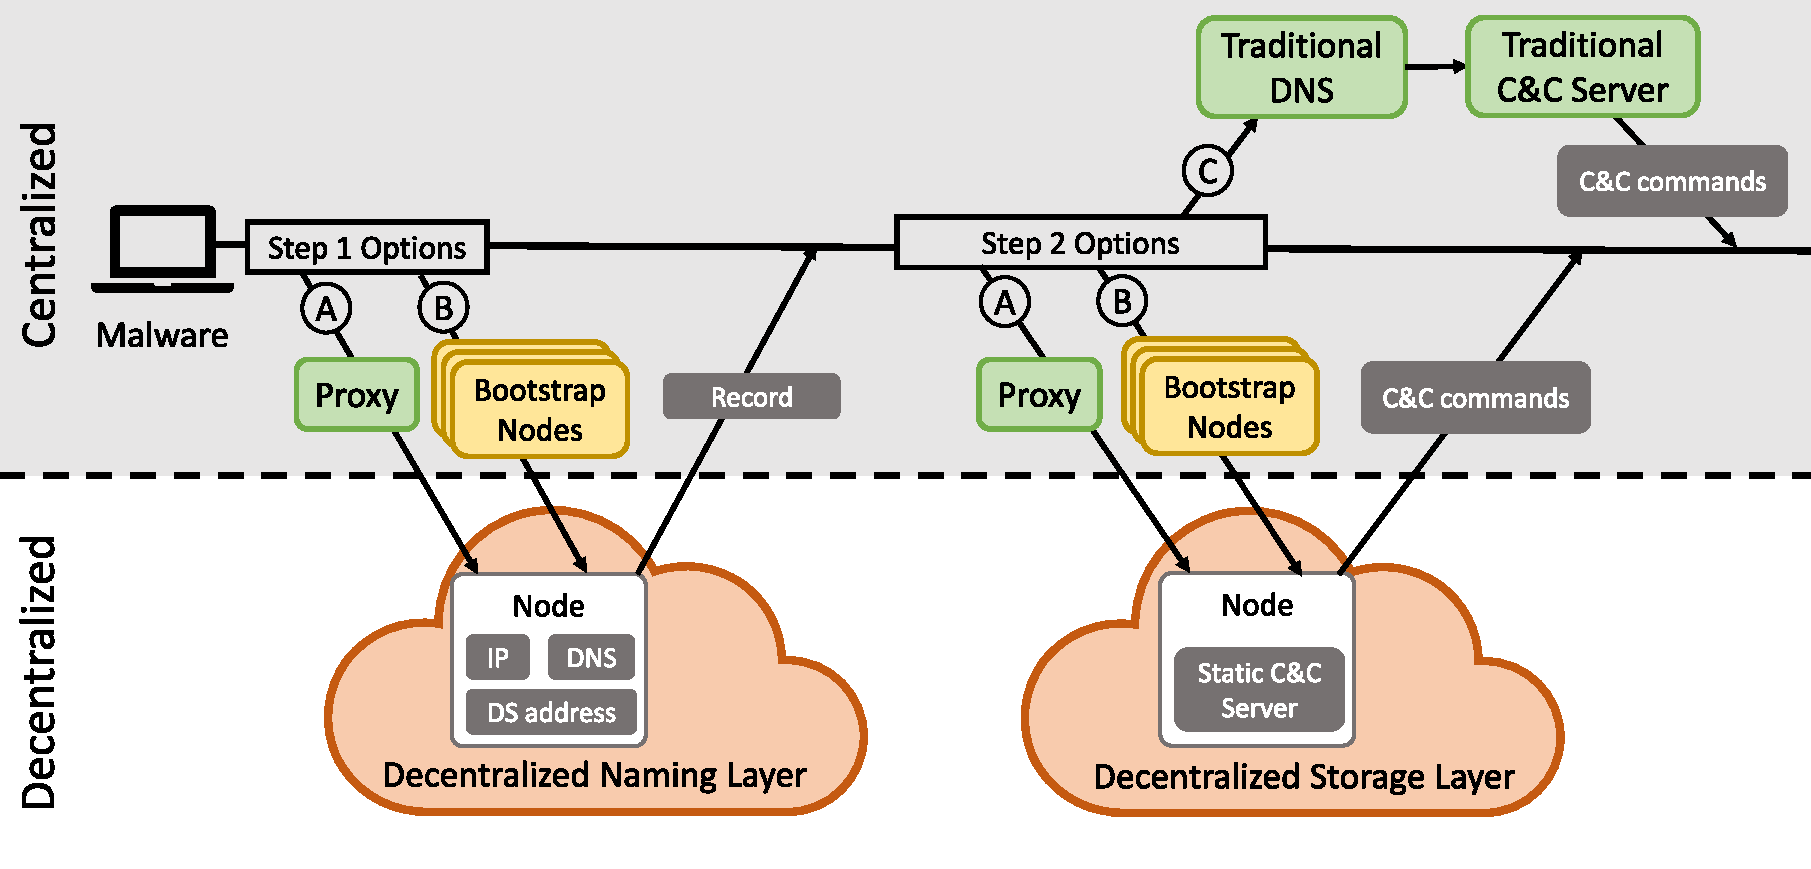
\includegraphics[width=\textwidth]{figs/malware_contacting_cnc.pdf}
	\caption{Malware must pass through centralized ``chokepoints'' to reach 
		decentralized systems, some of which might be good points for defender 
		interventions.}
	\label{fig:malware_contacting_cnc}
\end{figure*}

Anything in Figure~\ref{fig:malware_contacting_cnc} in green is centralized 
enough to have to respond to a takedown request. Anything in yellow is 
more difficult because taking it down would have collateral damage, and in 
orange it's probably impossible to take down because it's truly distributed and 
very resilient to takedowns.

Given that malware requires a naming layer and it’s useful to have it on a 
blockchain, it can access it in two ways (step 1 in 
Figure~\ref{fig:malware_contacting_cnc}:
\begin{itemize}
	\item Using a proxy: These are centralized, so still good points for 
	intervention. (Insert table of proxies we've found?)
	\item Being a first class member of a chain: You find the nodes using 
	bootstrap nodes then. These are challenging for defenders to take down bc 
	of collateral damage, but can be blocklisted by IDS, 
	enterprises, antivirus. 
\end{itemize}

Accessing a distributed, peer-to-peer system for the first 
time requires knowing the address of a participating node 
that is already connected to the system. In general, there 
are two methods for finding such an address: connecting to a 
proxy with a known domain or IP that is itself a full member 
of the system, or acting as a full member of the system 
yourself and utilizing the peer-to-peer discovery protocol 
used by all system nodes. The latter approach requires 
knowing a list of ``bootstrap nodes.'' A third option, a 
local discovery protocol that floods the network with 
messages looking for nodes, has not been adopted by any major 
blockchains that we are aware of. Such an approach would be 
very ``noisy'' and as such unlikely to be favored by malware, 
so we do not discuss it further.

\subsection{Accessing blockchains using proxies}

\begin{table}
	\begin{tabular}{r l l}
		\toprule
		Name system & TLDs & Proxies \\
		\midrule
		Namecoin & .bit & \\
		Emercoin & .lib, & PeerName,  \\
		& .bazar, & friGate, \\
		& .coin, & OpenNIC \\
		& .emc & \\
		Handshake & \emph{any string} & hns.to, \\
		& & NextDNS, \\
		& & HDNS.io,\\
		& & BobWallet extension, \\
		& & LinkFrame extension \\
		ENS & .eth & eth.link, \\
		& & eth.limo \\
		Unstoppable & .crypto, & Brave browser, \\
		& .blockchain, & Opera browser, \\
		& .bitcoin, & Unstoppable browser, \\
		& .coin, & Unstoppable extension, \\
		& .nft, & Infura\\
		& .wallet, & \\
		& .888, & \\
		& .dao, & \\
		& .x, & \\
		& .zil & \\
		\bottomrule
	\end{tabular}
	\caption{Non-exhaustive selection of proxies, browsers, 
	and extensions 
	that can be used to access blockchain-based naming 
	systems. \randall{maybe should have a citation for each 
	of these}}
	\label{tab:proxies_and_tlds}
\end{table}

To resolve a blockchain-based name, users have several choices. Most large 
browsers, such as Safari, Chrome, and Firefox, do not support any blockchain 
naming systems, but several extensions allow users to resolve names from ENS, 
Handshake, and Unstoppable Domains. These extensions rely on proxies that use 
DoH to send a resolution request to a server that can resolve the name. We 
note that such a server does not need to make a lookup to the chain every time 
it receives a request: it may cache names or keep track of its own database of 
names, which would simplify its implementation and speed up lookups 
significantly. 

Some browsers, such as Brave and Opera, claim to resolve certain naming systems 
natively. \randall{but when I tried this it didn't work? should try again with 
known websites and try Opera.} Both Brave and Opera rely on a proxy called 
Infura to resolve blockchain-based names. \randall{many citations needed.} 

Some naming systems have partnerships with existing DNS resolvers. For example, 
NextDNS and Handshake have partnered to allow users who set their DNS resolver 
to NextDNS to resolve Handshake domains. Finally, some naming systems, such as 
Handshake, also provide stub resolver implementations that run locally on a 
user's computer. 

As a side note, the existence of competing naming systems in which name 
collisions are possible 
opens up the possibility of collision-based attacks. There is no governance 
system in place to prevent different systems from adopting the same TLDs and 
causing name collisions. In fact, several collisions already exist, both 
between blockchain-based systems themselves (Emercoin and Unstoppable both 
provide a ``.coin'' TLD) and between ICANN TLDs and blockchain-based systems 
(both Handshake and ICANN provide ``.music''). 
This means the record that a user receives when resolving a name with a 
collision depends on which resolution method they use. If the user has multiple 
proxies set up --- for example, multiple browser extensions installed that each 
try to resolve domains with a specific TLD --- then the record received will 
depend on which of those proxies takes precedence, which is not at all clearly 
defined. 

Table~\ref{tab:proxies_and_tlds} provides a summary of the TLDs and proxies 
used by the blockchain naming systems we study. The list of proxies is not exhaustive, but 
represents 
a subset of the best-known proxies in use at the time of writing.
All of these proxies are 
centralized, which is good news for defenders: similarly to traditional 
registrars, they are vulnerable to legal takedowns. They can be served with 
legal takedown notices as long as they operate within a jurisdiction whose 
legal system is amenable to such efforts, or taken down through serving legal 
notices to their hosting providers. While these interventions are not 
bulletproof, they are subject to the same advantages and disadvantages as 
interventions on traditional registrars. Thus, centralized proxies return the 
distributed naming ecosystem to a state similar to the DNS ecosystem, from a 
defender's point of view. However, while proxies simplify the process of 
connecting to a blockchain, they are not strictly necessary, which is bad news 
for defenders.


\subsection{The emergence of light clients}

When blockchains were first envisioned, most assumed that every participant in 
the network would be a ``full'' implementation of a node: it would contain 
enough state to reconstruct the entire history of the chain, all the way back 
to the first transaction. Additionally, each node would contribute to the 
blockchain by verifying every transaction it heard about. As various 
blockchains have grown over time, they have become too resource-intensive to 
run on anything other than a dedicated, powerful machine. Two 
resources serve as 
the constraints: first, CPU power, which is obviously necessary to perform 
mining but now is even a bottleneck for transaction verification on some 
machines, because so many transactions happen per 
second~\cite{citation_needed}. Second, disk 
space and speed. For example, Ethereum cannot be run on a machine with a hard 
disk drive anymore, because nothing slower than an SSD can keep up with the 
reads and writes required~\cite{citation_needed}. \randall{I 
forget where I read this.} These resource constraints have 
given rise to the concept of a ``light client,'' a blockchain 
node with limited functionality that can fetch transactions 
from the chain but does not contribute by verifying 
transactions, mining, or broadcasting. Light clients are 
designed to run on laptops and mobile devices. As 
such, they are small enough to reasonably fit into a malware 
payload. 

Light clients enable malware to act as a first-class member 
of a blockchain, and discover other members of the chain 
using the chain's peer-to-peer discovery protocol without 
using a centralized proxy. Most peer-to-peer discovery 
protocols allow a client to connect to the blockchain for the 
first time by hard-coding a set of ``bootstrap nodes.'' In 
Ethereum, these bootstrap nodes are hard-coded into various 
implementations of the clients, and in Bitcoin, they are 
either hard-coded or accessible as TXT records stored at 
various trusted domains. The list of bootstrap nodes may also 
be configured by the user. If the 
malware chooses to use the bootstrap nodes that are 
hard-coded by default into the light client implementation, 
this may present a challenge for defenders, because taking 
down those bootstrap nodes may cause collateral damage to 
legitimate users attempting to join the chain. As such, 
bootstrap nodes are a more difficult place to stage an 
effective defender intervention than centralized proxies. 

\subsection{Naming record formats}

Once you've contacted the naming layer, you need to fetch the record that tells 
you how to get to your CNC server. 
The record stored in the naming layer can take 
several forms. The three that we saw were IP addresses, 
traditional domains, and links to distributed file storage 
systems like IPFS and SkyNet. It's theoretically possible 
that malware could store other types of records, like links 
to social media posts, too. All of these record types except 
for the DS addresses are subject to all of the usual 
interventions. Additionally, because all blockchain records 
are public, anyone can fetch those records including 
defenders. The DS addresses are the only new thing, so we'll 
focus on those next. Also, you can only use a DS address if 
your CNC server can be implemented as a static file.

Accessing a DS system is the same as accessing a distributed 
blockchain-based naming layer: you can do it either by proxy 
or by being a first-class member of the network, in which 
case you need bootstrap nodes. Theoretically, malware can go 
straight to the storage layer, but this is unlikely to be 
feasible given the way current DS systems are set up. The 
reason malware needs 
to use a naming layer to connect to the current generation of 
distributed file storage systems is because they're 
content-addressable. As soon as the file changes, so 
does its address, and the malware that knew the old address 
is useless. 
However, this is not a fundamental limitation of distributed 
storage systems --- a system could be designed in the future 
that doesn't have this limitation.

I don't know if IPFS/SkyNet have light nodes that could be 
part of a malware payload, but there does seem to be a trend 
in that direction as chains get heavier.

\section{Modifying records}

\subsection{Name-specific chains vs. general-purpose chains}

Name-specific chains, such as Namecoin, Emercoin, and 
Handshake, tend to have fewer participants, less popularity, 
and lower transaction fees. General-purpose chains, such as 
Bitcoin and Ethereum, have naming systems built on top of the 
underlying chain, such as ENS, Unstoppable Domains, and 
Blockstack. These chains have high transaction or gas fees 
and the names are more expensive to buy (except haven't 
checked Blockstack). 

\subsection{Challenges on general-purpose chains}

\begin{itemize}
	\item High monetary cost of txns
	\begin{itemize}
		\item Defenders can't pre-register DGA domains
		\item But for malware authors, making fast flux work 
		is harder. 
	\end{itemize}
	\item Blocking malware's access to the chain
	\begin{itemize}
		\item Can't just keep every computer on the Internet 
		from accessing the chain, via IDS or whatnot, because 
		too many legit users.
	\end{itemize}
	\item \randall{Where do I put this?} Seizing control of 
	the wallet that owns a domain: 
	What about hosted wallets? If malware authors are using 
	hosted wallets to own the blockchain DNS domains, the 
	hosting service like Coinbase could presumably seize 
	them, because it has the private keys. The solution is 
	just to not use hosted wallets, but is that possible with 
	the way ENS and UD are set up? Even if it's hard, you 
	could transfer the domains to a non-hosted wallet as soon 
	as you make them. So probably not a good intervention 
	point, too easy to evade. 
\end{itemize}

\begin{figure}[t]
	\centering
	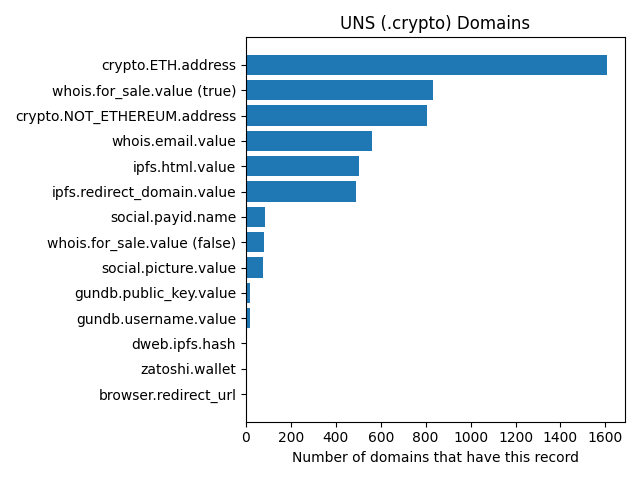
\includegraphics[width=3in]{uns_records.png}
	\caption{Types of records stored by Unstoppable 
	Domains with TLDs other than .crypto}
	\label{fig:uns_records}
\end{figure}
\begin{figure}[t]
	\centering
	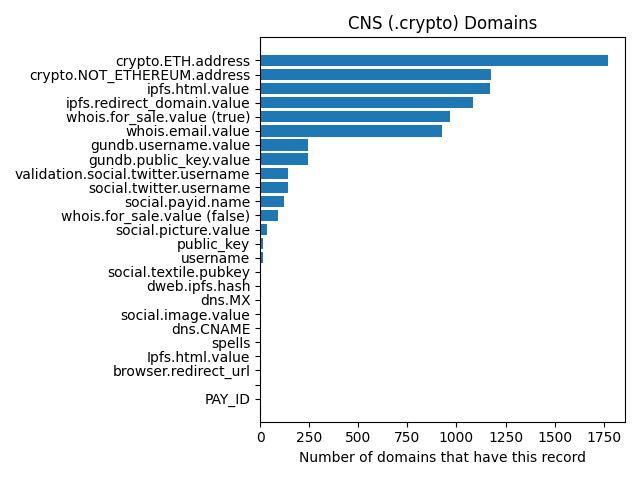
\includegraphics[width=3in]{cns_records.png}
	\caption{Types of records stored by Unstoppable Domains 
	with .crypto TLDs}
	\label{fig:cns_records}
\end{figure}


Now let's describe the specific chains in more detail. These 
systems are advertised differently - they mostly store 
wallet address records even though they're set up like DNS, 
with registrars and registries. 

\subsubsection{ENS}

Describe the registrar/registry/resolver structure.

Haven't found anything bad yet except loli-hentai.eth. This 
system, like all other uncensorable systems, will probably 
eventually attract CSAM. Describe what we did to find 
domains, how I crawled a subset.

\subsubsection{Unstoppable Domains}

Describe the registry contract and the crawled domains (I did 
crawl these didn't I?)

We don't think malware is using large chains yet because of 
the high cost of txns. If the cost goes down, or defenders 
block/take down the cheaper alternatives, malware might be 
forced to use the large chains. However, malware still seems 
to be using the small chains (Namecoin and Emercoin) a lot.

\section{Challenges on small chains}
\begin{itemize}
	\item High txn cost is less of an issue: defenders might 
	be able to register DGA domains? 
	\item Blocking the whole thing using antivirus and 
	middleboxes, or taking the whole thing down, is probably 
	possible, because there's so few legit users. Even that 
	one proxy stopped serving access to .bit domains. A 51\% 
	attack is possible on Namecoin because one pool already 
	had ~60\% of the hashing power. Also possible just to 
	blocklist every IP recorded in the chain's domain records.
\end{itemize}

The vast majority of names in ENS, Unstoppable, and Handshake 
don't have records because it's so hard to set them up, and 
while you can buy the records with no technical knowledge you 
can't assign records to them without writing code afaict. 
Also, people are mostly using these as speculative assets, 
which is another reason plenty of them have no records.

\subsection{Namecoin and Emercoin}

Plenty of DGA .bit stuff in the b-root leakage, so malware is 
still using Namecoin for sure. Should check the diffs between 
the old and new B-root dumps (numbers of hits for each TLD, 
etc)

Cite/summarize those two papers that found all sorts of 
nastiness on these chains.

\subsubsection{Handshake}

Handshake is a new blockchain-based system that aims to 
replace the root DNS 
zone. As such, it offers its users the ability to purchase 
nearly any string to 
use as a TLD. Rather than selling second-level domains 
itself, the Handshake ecosystem purports to allow its users 
to act as registrars who can sell their own domains. 
Handshake's stated goal is not to replace the traditional DNS 
system: Handshake records are designed to store the domains 
and IP addresses of traditional authoritative nameservers, 
rather than to store A, AAAA, or CNAME records. However, 
Handshake also allows users to store TXT records, which can 
contain the addresses for decentralized web hosting systems 
like Skynet or IPFS. Malware users could therefore use 
Handshake as a naming system to find content stored in 
content-addressed distributed storage systems.

``Handshake is the only naming blockchain with a lightweight 
recursive DNS resolver, which you can easily embed into 
browsers, apps, and devices.'' - 
https://learn.namebase.io/starting-from-zero/how-to-access-handshake-sites
So it can use the bootstrap nodes and participate in 
Handshake as a first class citizen, which is challenging for 
defenders.

Handshake stats:
\begin{itemize}
	\item The vast majority of names just have two GLUE4 
	records with two nameservers: “ns1.name” and “ns2.name”. 
	The IPs in these glue4 records are 44.231.6.183 and 
	54.214.136.246, respectively.
	\item Many of the most expensive TLDs (.x, .crypto, .js, 
	.8, .wallet) return an SOA record pointing to 
	``a.misconfigured.powerdns.server''
	\item ~100K had a nameserver record (all of them pointed 
	to what I assume is the Namebase resolver, except one or 
	two.) Out of those 100,000, only 101 actually had an A 
	record. 94/100 point to one IP address: 44.235.163.135. 
	That's an AWS IP that gives a 404 if you visit it with a 
	browser. Four more point to 52.43.158.89 (another AWS 
	IP), which redirects to an unconfigured distributed 
	hosting provider site. One points to 1.1.1.1, and two 
	look like someone's unconfigured personal website.
\end{itemize}

\section{What might cause a naming system to present a threat?}

What would cause a decentralized naming system to be popular enough that 
defenders wouldn't want to block access to it?
\begin{itemize}
	\item Ease of use: owners don't have to write code
	\item Affordable txns
	\item Widespread browser adoption
\end{itemize}

%\section{How big of a threat is blockchain DNS?}
%The original goal of this paper was to say whether malware 
%using blockchain to 
%contact its C\&C servers was actually a huge threat. We can 
%approach this 
%problem in two ways: (1) Map out the ecosystem and say 
%whether it's POSSIBLE, 
%(2) Check the current records being stored and say whether 
%it's already 
%happening.
%
%\section{Whether it's possible}
%
%We haven't yet started up an Ethereum light node to see if 
%it could be part of 
%a malware payload. 
%
%Stefan originally thought that because PCs/phones can't be 
%first class 
%blockchain citizens, malware won't be able to connect to a 
%blockchain without 
%using a proxy. The proxy would be an intervention point for 
%defenders to say, 
%stop serving this stuff, we have a court order. The 
%assumption there is that 
%malware can't connect to a blockchain without using a proxy. 
%I think that's 
%incorrect because the Ethereum nodes themselves use a 
%Chord-like protocol, 
%Kademlia, which I assume-but-need-to-check is a thing where 
%one node knows more 
%nodes, which know more nodes, etc. 
%
%Kademlia relies on bootstrapping, and in fact, the Ethereum 
%nodes out there 
%supposedly get their node lists from a set of bootstrap 
%nodes. You probably 
%can't outright take down the bootstrap nodes, because that 
%breaks new nodes 
%connecting to Ethereum. 
%
%Start with the simplest case - hard-coded Ethereum node 
%domains/IPs. That isn't 
%any better than just having hard coded domains/IPs of your 
%C\&C server, because 
%they're still easy for defenders to block. The caveat is, 
%maybe defenders don't 
%want to take down innocent Ethereum nodes? Because they 
%serve another, benign, 
%purpose besides malware. Stefan thinks defenders wouldn't 
%hesitate to take down 
%nodes that were hard-coded as malware access points to 
%Ethereum. But what if 
%those nodes were the official bootstrap nodes? Defenders 
%wouldn't want to take 
%those down.
%
%\subsection{Light nodes}
%
%Is it enough to just do the PING-PONG and then try to sync 
%txns? I mean, all of 
%that will be much easier if you use a light client, but 
%could you even pull 
%that code out and do it yourself? Or will the full nodes 
%say, nah we don't want 
%to connect to you? 

%Stefan was wondering which Ethereum nodes are actually used 
%for transactions, 
%and whether there's an even distribution or some nodes are 
%taking all the 
%strain. I wonder if you could say, lots of ppl are making 
%txns using Infura's 
%full nodes, let's block those txns from going out onto the 
%network? If no one 
%else can verify them, they can't get added. Or you could 
%DDoS 
%a full node to 
%prevent it sending out the message that says it's mined the 
%next block, but I'm 
%sure someone has thought of that attack already.
%
%\section{Extra interesting stuff we found along the way}
%
%\subsection{Typo squatting}


\bibliographystyle{ACM-Reference-Format}
\bibliography{references}

%\appendix
%\section{Ethics}
%
%This work raises no ethical concerns.

\end{document}
